\section{Connected two-point reductions and the native index limit}
\label{sec:notes-prop-tree}
The preceding triangle identity suggests a further reduction: a connected tree of massless bubbles also closes analytically when its root is a two-point integral. We implement this extension before the existing analytic and learned choices. It recognizes the momenta, masses, and powers, integrates each nonroot bubble, and evaluates the remaining root bubble. The dimension-dependent powers transferred between subintegrals are retained exactly. Appendix~\ref{app:notes-prop-tree} defines the family and derives the rational target-to-master coefficient. This use of massless subintegrals follows established parametric propagator methods~\cite{Ruijl2017Forcer}.

This extension also clarifies the apparent loop limit. Kira requires a complete set of $N=L(L+1)/2+LE$ scalar-product coordinates for $L$ loops and $E$ independent external momenta~\cite{Kira3}. The installed native build rejects more than 31 indices, including auxiliary scalar-product coordinates. Consequently, its complete-coordinate limit is seven loops for vacuum families, six for two-point families, and five for families with two or three independent external momenta. Appendix~\ref{app:notes-prop-tree} derives the coordinate count. Exact integration bypasses this native input within the stated analytic domain; it does not remove the restriction for an arbitrary remaining graph.

We freeze 34 distinct two-point tree structures with seven targets each, covering every loop order from one through thirteen. Their scale remains symbolic. Three fresh processes compare the extended application with the preceding application under a twelve-second limit per call. Sixteen triangle requests check the unchanged exact path, while sixteen native two-loop box requests also compare the retained trained choices with fixed choices. The complete timer includes startup, recognition, coefficient calculation or native reduction, model evaluation when used, output, and exit. Independent checks follow timing on both sides.

All 34 two-point requests complete with the new rule. The preceding application completes 3 in every repetition. Among its 31 unsuccessful requests, 21 exceed the native index limit, nine reach the application deadline, and one fails the master-basis verification. We retain these failures in the completion counts and calculate speed ratios only from matched completed requests. The reserved two-point targets pass 714 independent Gamma checks at 80-digit precision and scaled error tolerance $10^{-60}$. Development also supplies 9 exact coefficient comparisons with native Kira. These checks test the derived identity; the high-loop results do not represent native high-loop IBP solves.

\begin{table}[!htbp]\centering\small
\caption{Complete times from sums of three-run request medians. The completion columns count requests completed in all repetitions. Times use only requests completed by both methods. The ML row uses fixed native choices as its control.}
\label{tab:notes-prop-tree}
\begin{tabularx}{\linewidth}{@{}Yrrrr@{}}\toprule
Comparison & Control/new complete & Paired & Control (s) & New (s)\\\midrule
Two-point trees & 3/34 & 3 & 11.185 & 0.433 \\
Triangle checks & 16/16 & 16 & 2.557 & 2.593 \\
Native path checks & 16/16 & 16 & 48.719 & 48.941 \\
Retained ML versus fixed & 16/16 & 16 & 52.226 & 48.941 \\
\bottomrule\end{tabularx}\end{table}

For the 3 matched two-point requests, total time falls from 11.185 to 0.433 seconds, a reduction of 96.1\%. The time ratio is 0.039, with a request-resampling interval of $[0.015,0.859]$. Across all 35 matched requests in this comparison, time changes from 62.461 to 51.967 seconds. The analytic extension accounts for the new two-point gain. No new ML model is fitted for this identity.

The matched collection-wide ratio is 0.832, with request interval $[0.569,1.010]$. This interval includes equal time, so the collection-wide point estimate does not establish a gain across integral families. The unchanged triangle and native paths also have intervals that include equal time.

On the sixteen native requests, the retained learned choices take 48.941 seconds against 52.226 seconds for fixed choices, giving ratio 0.937 and request-resampling interval $[0.853,1.010]$. The trained batch policy runs on all sixteen requests, choosing the wider sparse seed setting thirteen times and the tighter setting three times. This fresh comparison does not resolve a reliable ML gain because the interval includes equal time. The earlier controlled seed and equation-selection gains remain separate evidence. The new two-point reduction retains the preceding ML policy for its eligible native inputs. It supports the specified connected massless trees and preserves the documented failures for general massive, multiscale, and irreducible scattering families.

\begin{figure}[!htbp]\centering
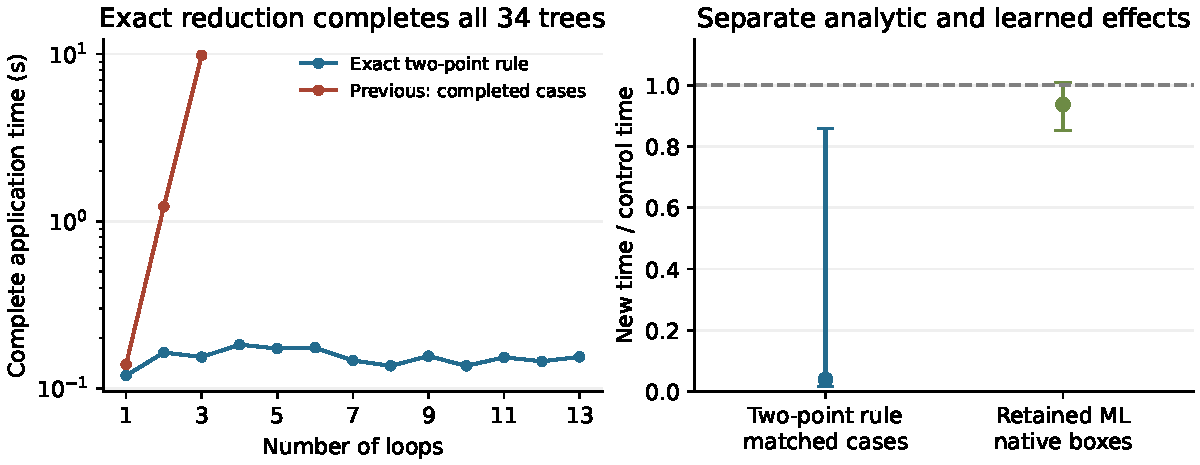
\includegraphics[width=\linewidth]{paper_figures/propagator_trees.pdf}
\caption{The exact rule completes the defined two-point trees through thirteen loops. The left panel uses a logarithmic time axis and averages request medians at each loop order. Control points include completed requests only; missing points have no completed control and imply no finite speed factor. The right panel separates the exact extension from the retained native ML contribution, using matched completed requests and request-resampling intervals.}
\label{fig:notes-prop-tree}
\end{figure}
\FloatBarrier
